\section{Experiments}\label{sec:eval}

% \ds{The section looks good overall.  I made only stylistic changes,
%   mostly in the beginning.  Regarding the Latex layout, I don't
%   onecolumn should be the solution, but instead you should use a
%   figure$*$, then subfigures.  Also, I think you can squeeze in
%   another graph, i.e. arrange them $3 \times 3$.}

We implemented \FJ as a standalone Rust library.  The main entry point
of the library is a function that takes a binary join plan (produced
and optimized by DuckDB), and a set of input relations.  The system
converts the binary plan to a \FJ plan, optimizes it, then runs it
using \COLT and vectorized execution.
%%% The binary plan can be produced by any query optimizer, and we
%%% convert the binary plan into a \FJ plan and further optimize it as
%%% described in Section~\ref{sec:bj-to-fj}.
% In addition to joins, our implementation supports 
%   projection and aggregation, 
%   but relies on an external system for selection.
We compare \FJ against two baselines: our own \GJ implementation in
Rust, and the binary hash join implemented in the state-of-art
in-memory database
DuckDB~\cite{DBLP:conf/cidr/RaasveldtM20,DBLP:conf/vldb/Raasveldt22}.
We evaluate their performance on the popular Join Order Benchmark
(JOB)~\cite{DBLP:journals/pvldb/LeisGMBK015}.
We refer the reader to our SIGMOD paper~\cite{10.1145/3589295}
for additional experiments that include other systems
and benchmark, as well as detailed ablation studies of the optimizations.


% \clearpage
% \onecolumn
\subsection{Setup}

While we had easy access to optimized join plans produced by DuckDB,
we did not find any system that produces optimized \GJ plans,
or can take an optimized plan as input.
%%% 
%%% In addition to using DuckDB as a baseline implementation of binary
%%% join, we use its query optimizer to generate the starting binary plan
%%% that we convert into a \FJ plan.
%%% %
%%% Compared to binary join implementations, 
%%%   there are few systems that implement \GJ, 
%%%   and none of them outputs a machine-readable query plan,
%%%   or can take one as input.
We therefore implement a \GJ baseline ourselves,
by modifying \FJ to fully construct all tries, and removing
vectorization.  We chose as variable order for \GJ the same as for
\FJ.\footnote{\FJ defines only a partial order; we extended it to a
  total order.}

%%% It is essentially \FJ but without the optimizations:
%%%   its execution is not vectorized, and
%%%   instead of using \COLT, it fully constructs every trie ahead of time.
%%% We are not aware of any other algorithm converting a binary plan into a \GJ plan, 
%%%   so we use the same plan for both \FJ and \GJ to ensure a fair comparison.

The JOB benchmark contains 113 acyclic join queries with an average of 8 joins per query.
Each query in the benchmarks only contains base-table filters,
natural joins, and a simple group-by at the end,
and no null values.
The queries works over real-world data from the IMDB dataset.
We exclude 5 queries that return empty results,
since such empty queries are known to introduce reproducibility issues\footnote{
  See GitHub issue: https://github.com/gregrahn/join-order-benchmark/issues/11
}.

We ran all our experiments on a MacBook Air laptop with Apple M1 chip and 16GB memory.
All systems are configured to run single-threaded in main memory,
and we leave all of DuckDB's configurations to be the default.
All systems are given the same binary plan optimzed by DuckDB.
Since we are only interested in the performance of the join algorithm,
we exclude the time spent in selection and aggregation
when reporting performance.
This excluded time takes up on average less than 1\% of the total execution time.

\begin{figure}
  \centering
  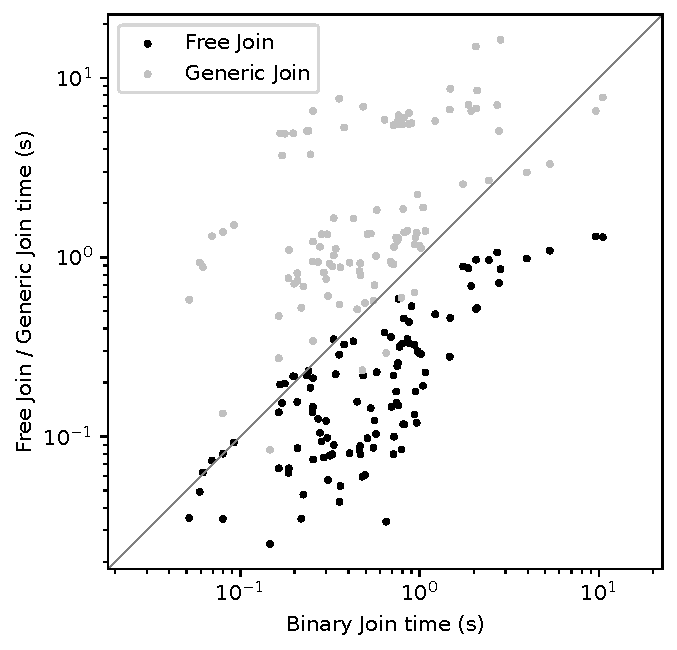
\includegraphics[width=.9\linewidth]{imdb.pdf}
  \captionof{figure}{Run time comparison on JOB.
    Each black dot compares the run time of a query on \FJ and binary join,
    and a black dot below the diagonal means \FJ is faster.
    The gray dots compare \GJ and binary join similarly.
  }
  \label{fig:eval:imdb}
\end{figure}%

\begin{figure}
  \centering
  \begin{tabular}{c}
    \begin{lstlisting}[numbers=none]
111101
JOIN
 |  \________9775
1919495      company_name(cid)
JOIN
 |  \________1
8123586      company_type(ctid)
JOIN
 |  \________1
24740873     info_type1(iid1)
JOIN
 |  \________1
148621556    info_type2(iid2)
JOIN
 |  \________1
177388547    kind_type(kid)
JOIN
 |  \________2609129
20885030     movie_companies(mid, cid, ctid)
JOIN
 |  \________1380035
 |           JOIN
 |            |  \_____1380035
 |           2528312   movie_info_idx(mid, iid1)
 |           title(mid, kid)
14835720    
movie_info(mid, iid2) 
\end{lstlisting}
  \end{tabular}
  \caption{Query plan produced by DuckDB for JOB Q13a.
    We show the join attributes next to each input relation,
    and label each relation with its size as well as
    each join with its (actual) cardinality.  }
  \label{fig:eval:imdb:plan}
\end{figure}


% \end{lstlisting}
% \end{figure*}

% \begin{figure*}
%   \centering
%   \begin{minipage}[t]{.45\textwidth}
%     \centering
%     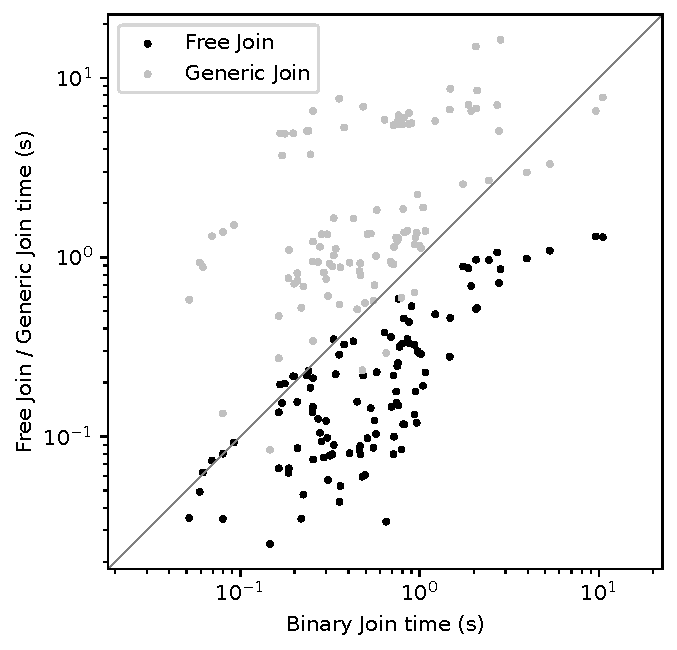
\includegraphics[width=\linewidth]{imdb.pdf}
%     \captionof{figure}{Run time comparison on JOB.
%       Each black dot compares the run time of a query on \FJ and binary join,
%       and a black dot below the diagonal means \FJ is faster.
%       The gray dots compare \GJ and binary join similarly.
%     }
%     \label{fig:eval:imdb}
%   \end{minipage}%
%   \hspace{1em}
%   \begin{minipage}[t]{.45\textwidth}
%     \centering
%     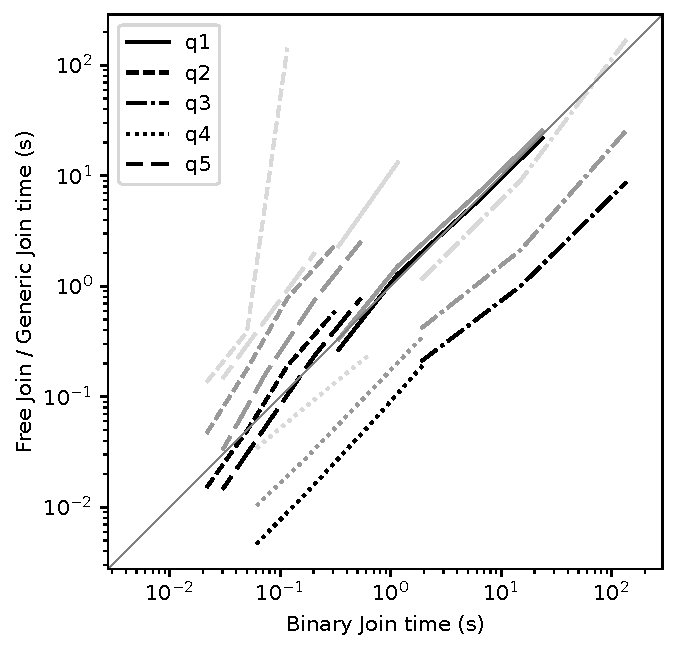
\includegraphics[width=\linewidth]{lsqb-slow.pdf}
%     % \captionof{figure}{\FJ and \GJ v.s.\ binary join on LSQB queries.
%     % Each line is a query running on increasing scaling factors (0.1-3).
%     % Grey lines are for \GJ, and black lines are for \FJ.
%     % }
%     \captionof{figure}{Run time comparison on LSQB.
%       Each line is a query running on increasing scaling factors (0.1, 0.3, 1, 3).
%       The black lines compare \FJ with binary join,
%       the gray lines compare our \GJ baseline with binary join,
%       and the light gray lines compare K\`uzu with binary join.
%     }
%     % Grey lines are for \GJ, and black lines are for \FJ.
%     % }
%     \label{fig:eval:lsqb}
%   \end{minipage}
% \end{figure*}


\subsection{Run time comparison}\label{sec:run-time-comparison}

Figure~\ref{fig:eval:imdb} compares the run time of \FJ and \GJ against binary join on JOB queries.
We see that almost all data points for \FJ are below the diagonal,
indicating that \FJ is faster than binary join.
On the other hand, the data points for \GJ are largely above the diagonal,
indicating that \GJ is slower than both binary join and \FJ.
On average (geometric mean), \FJ is \imdbavgfjbj faster than binary join
and \imdbavgfjgj faster than \GJ.
The maximum speedups of \FJ against binary join and \GJ
are \imdbmaxfjbj and \imdbmaxfjgj, respectively,
while the minimum speedups are \imdbminfjbj (\imdbmaxbjfj slowdown) and \imdbminfjgj.

We zoom in onto a few interesting queries for a deeper look.
The slowest query under DuckDB is Q13a, taking over 10 seconds to finish.
\GJ runs slightly faster, taking 7 seconds,
whereas \FJ takes just over 1 second.
The query plan for this query,
as shown in Figure~\ref{fig:eval:imdb:plan},
reveals the bottleneck for binary join:
the first 3 binary joins are over 4 very large tables,
and two of the joins are many-to-many joins, exploding the
intermediate result to contain over 100 million tuples.
However, all 3 joins are on the same attribute (\lstinline|mid|);
in other words they are quite  similar to our clover query $Q_\clubsuit$.
As a result, \GJ and \FJ simply intersects the relations
on that join attribute,
expanding the remaining attributes only after
other more selective joins.
% This data point appears to confirm a folklore that claims
% \WCOJ algorithms are more resistant to poor query plans.
% After all, binary join could have been faster, had the query plan
% ordered the more selective joins first.
% We expand on this point with more experiments evaluating
% each algorithm's robustness against poor plans in Section~\ref{sec:robustness}.

On a few queries \FJ runs slightly slower than binary join,
as shown by the data points over the diagonal.
The binary plans for these queries are all bushy,
and each query materializes a large intermediate relation.
We have not spent much effort optimizing for materialization,
and we implement a simple strategy: for each intermediate
that we need to materialize, we store the tuples containing
all base-table attributes in a simple vector.
Future work may explore more efficient materialization strategies,
for example only materializing attributes that
are needed by future joins.

% Figure~\ref{fig:eval:lsqb} compares the performance of \FJ and \GJ against binary join on LSQB queries.
% Each line corresponds to one query running on scaling factors 0.1, 0.3, 1, and 3.
% The black lines are for \FJ, gray lines for our own \GJ baseline, and light gray lines for K\`uzu.
% K\`uzu errors when loading data for SF3;
% it did not finish after 10 minutes for q1 SF 1.
% DuckDB also took over 10 minutes running q3 SF 3.
% These instances do not show up in the figure.
% We can see K\`uzu takes consistently longer than our \GJ implementation
% on all queries across scaling factors.
% This shows that our \GJ implementation is a reasonable baseline to compare against.
% On cyclic queries, \FJ is up to 15.45x (q3) faster than binary join,
% and up to 4.08x (q2) faster than \GJ.
% On acyclic queries \FJ is up to 13.07x (q4) and 3.25x (q5) faster than binary join and \GJ, respectively.
% On q3 and q4 both \FJ and \GJ consistently outperform binary join on all scaling factors.
% q3 contains many cycles, whereas q4 is a star query, so the superior performance of \FJ and \GJ is expected.
% % q1, however, is a chain query, where \WCOJ algorithms are expected to be inefficient.
% % A deeper look reveals q1 to have an output much larger than its inputs, 
% %   but uses a \lstinline|COUNT(*)| at the top.
% % An unintended benefit of \GJ and \FJ is that any attributes that 
% %   do not participate in a join are not expanded, 
% %   so the output result is naturally stored in a \emph{factorized} form.
% % We compute the \lstinline|COUNT| aggregate directly on the factorized output, 
% %   which is much faster than expanding and counting.
% Surprisingly, despite q2 being a cyclic query,
% \FJ is only slightly faster on smaller inputs
% and is even slightly slower on larger inputs.
% This is the opposite of the common believe that \WCOJ algorithms
% should be faster on cyclic queries.
% The query plan reveals that there are no skewed joins,
% and so binary join suffers no penalty.
% Our experience shows that, in practice,
% the superiority of \WCOJ algorithms like \FJ and \GJ
% is not solely determined by the cyclicity of the query;
% the presence of skew in the data is another important factor.

% \begin{figure}
%   \centering
%   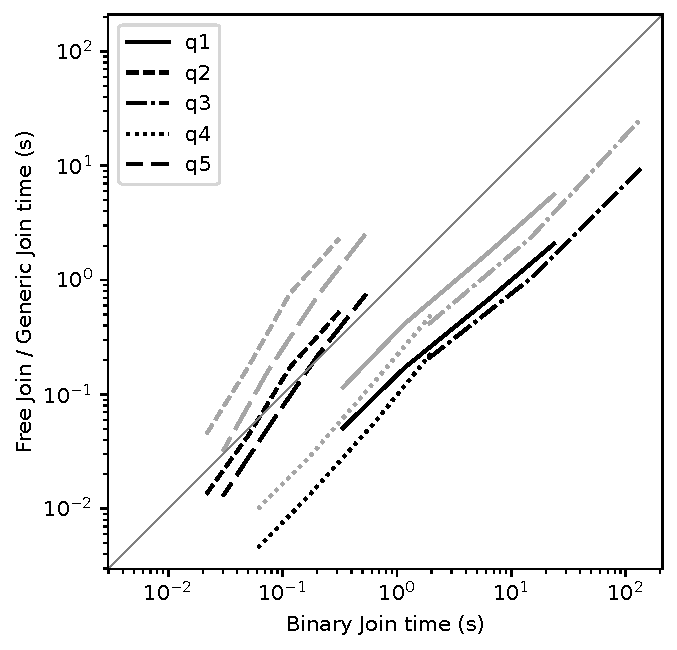
\includegraphics[width=.45\linewidth]{lsqb.pdf}
%   \caption{Run time comparison on LSQB w/ factorization.}
%   \label{fig:eval:lsqb-factor}
% \end{figure}

% Unlike the JOB queries, in LSQB the output size (before aggregation)
% is much larger than the input size.
% This leads to a large amount of time spent in constructing the output,
% which involves random accesses to retrieve the data values for each tuple.
% We therefore implemented the optimization in Section~\ref{sec:fj-gj-multijoin}
% to factorize the output.
% This made q1 significant faster, as shown in Figure~\ref{fig:eval:lsqb-factor},
% while other queries are not affected.

% \begin{figure*}
%   \centering
%   \begin{minipage}{.45\textwidth}
%     \centering
%     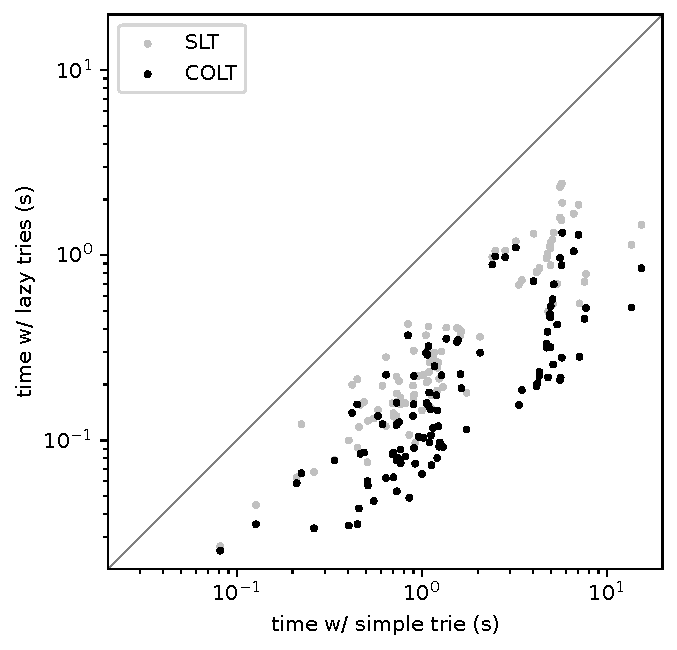
\includegraphics[width=\linewidth]{colt-ab.pdf}
%     \captionof{figure}{Impact of \COLT.}
%     \label{fig:eval:colt-ab}
%   \end{minipage}%
%   \hspace{1em}
%   \begin{minipage}{.45\textwidth}
%     \centering
%     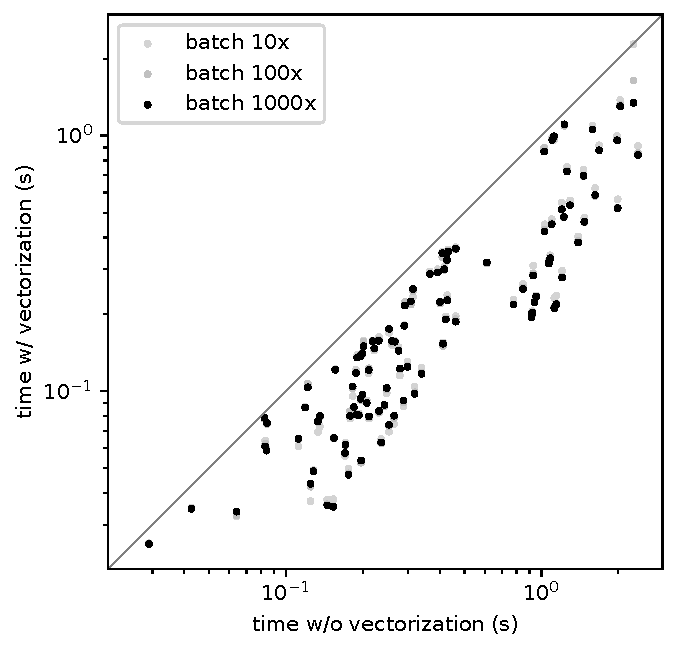
\includegraphics[width=\linewidth]{vec-ab.pdf}
%     \captionof{figure}{Impact of vectorization.}
%     \label{fig:eval:vec-ab}
%   \end{minipage}
% \end{figure*}
% % \subsection{Impact of \COLT and Vectorization}
% % % \ds{Try to choose section titles that are related to the question
% % %   that the section addresses}
% % The three key ingredients that make \FJ efficient
% % are \begin{enumerate*}
% %   \item our algorithm to optimize the \FJ plan by factoring,
% %   \item the \COLT data structure, and
% %   \item the vectorized execution algorithm.
% % \end{enumerate*}
% % We conduct an ablation study to evaluate the performance impact of these components.
% % But if we do not optimize the \FJ plan converted from a binary plan
% % and execute it as-is, \FJ would behave identically to binary join.
% % Since we have already compared \FJ with binary join in Section~\ref{sec:run-time-comparison},
% % we do not repeat it here.
% % Therefore, our ablation study includes two sets of experiments,
% % evaluating the impact of \COLT and vectorization respectively.



% Figure~\ref{fig:eval:colt-ab} compares the run time of \FJ using different trie data structures.
% The baseline fully expands each trie ahead of time, and we call this \emph{simple trie}.
% Another data structure, \emph{simple lazy trie} (SLT), expands the first level of each trie
% ahead of time, while expanding the inner levels lazily.
% This is the same strategy as proposed by Freitag et.al.~\cite{DBLP:journals/pvldb/FreitagBSKN20}.
% Finally, \COLT is our column-oriented lazy trie.
% In all three cases, we use the default vectorization batch size 1000.
% The experiments show the average (geometric mean) speedup of \COLT
% is 1.91x and 8.47x, over SLT and simple trie respectively,
% and the maximum speedup over them is 11.01x and 26.29x, respectively.


% Figure~\ref{fig:eval:vec-ab} compares the run time of \FJ using different vectorization batch sizes.
% The baseline uses no vectorization, i.e., we set the batch size to 1.
% Then we adjust the batch size among 10, 100, and 1000.
% The data does not show significant performance differences among
% the different batch sizes --
% it appears \emph{any amount of vectorization is better than none}.
% For short-running queries, a smaller batch size perform slightly better,
% and for longer running queries a larger batch size wins.
% We conjecture this is due to a smaller batch having less overhead,
% leading to lower latency,
% while a larger batch size speeds up large joins better,
% leading to better throughput.
% Overall, using the default batch size 1000
% leads to an average (geometric mean) speedup of 2.12x,
% and a maximum speedup of 5.33x over non-vectorized \FJ.

% \begin{figure*}
%   \begin{minipage}{.45\textwidth}
%     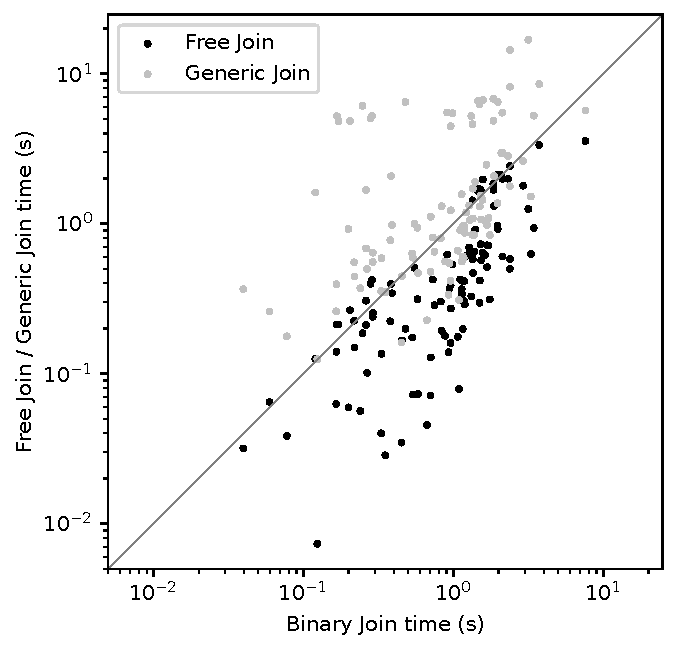
\includegraphics[width=\linewidth]{robust.pdf}
%   \end{minipage}
%   \hspace{1em}
%   \begin{minipage}{.45\textwidth}
%     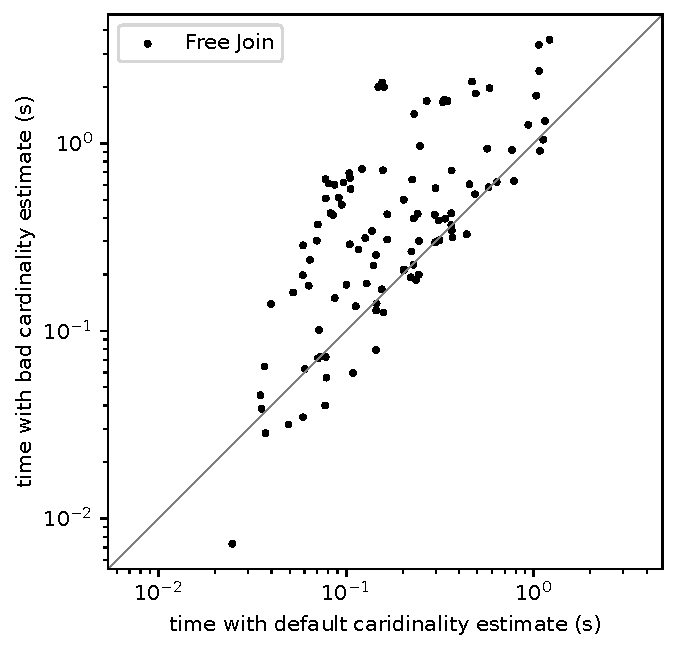
\includegraphics[width=\linewidth]{robust_fj.pdf}
%   \end{minipage}
%   \begin{minipage}{.45\textwidth}
%     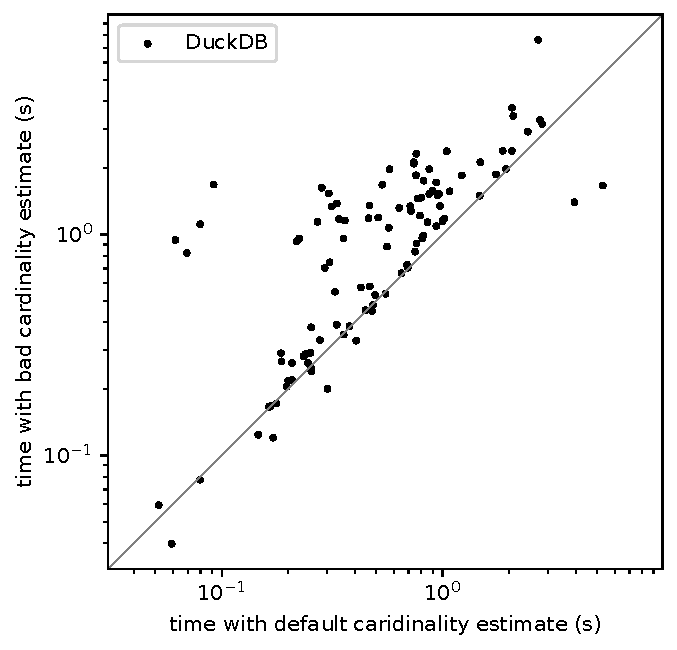
\includegraphics[width=\linewidth]{robust_bj.pdf}
%   \end{minipage}
%   \hspace{1em}
%   \begin{minipage}{.45\textwidth}
%     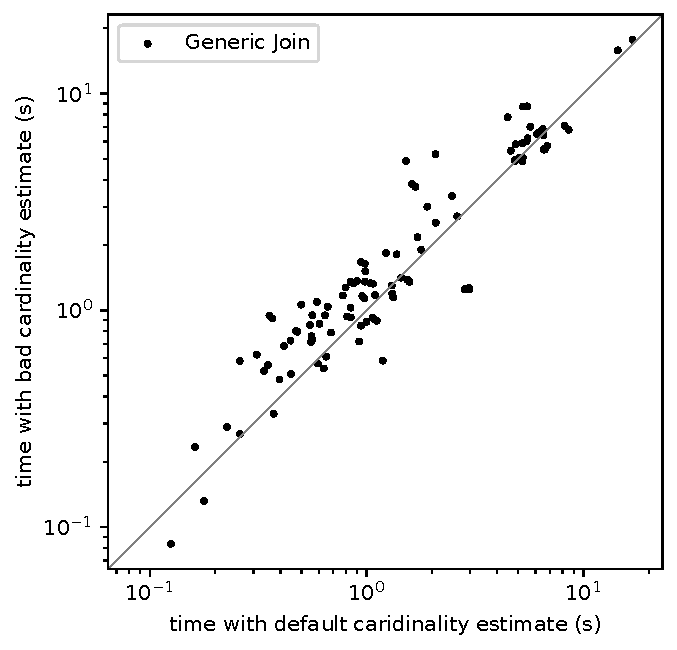
\includegraphics[width=\linewidth]{robust_gj.pdf}
%   \end{minipage}
%   \caption{Run time of join algorithms with good and bad cardinality estimates.
%     The first plot compares the run time of \FJ, \GJ and binary join
%     on JOB with bad cardinality estimates.
%     The remaining three plots compare the run time of each algorithm
%     with good and bad cardinality estimates on JOB.
%   }
%   \label{fig:sensitivity}
% \end{figure*}

% \subsection{Robustness Against Poor Plans}\label{sec:robustness}

% Our last set of experiments compares \FJ, \GJ and binary join
% on their sensitivity to the quality of the query plan.
% Many believe \WCOJ algorithms suffer less from poor query planning,
% due to its asymptotic guarantees.
% Our experience with Q13 from Section~\ref{sec:run-time-comparison}
% also seems to confirm this intuition.
% However, our experimental results tell a different story.
% As the first plot in Figure~\ref{fig:sensitivity} shows,
% the relative performance of the three algorithms stays
% the same with good and bad plans, with \FJ being the fastest,
% \GJ the slowest, and binary join in the middle.
% However, as shown in Figure~\ref{fig:sensitivity},
% \FJ seems to slow down as much as binary join
% when the plan is bad (there are many points far above the diagonal).
% It turns out with a poor cardinality estimate,
% DuckDB routinely outputs bushy plans that materialize large results.
% We have noted in Section~\ref{sec:run-time-comparison} that
% our materialization strategy is simplistic,
% so with larger intermediates it leads to more severe slowdown.
% In comparison, \GJ slows down less (the data points are close to the diagonal).
% However, it was the slowest to begin with,
% and since overheads like trie building dominates \GJ's run time,
% a bad plan does not make it much slower.
% Overall, we believe \FJ can be more robust to bad plans with
% faster materialization.
